\documentclass{scrreprt}
\usepackage{listings}
\usepackage{underscore}
\usepackage[bookmarks=true]{hyperref}
\usepackage[utf8]{inputenc}
\usepackage[english]{babel}
\usepackage{tikz}
\usepackage{xcolor}
\usepackage{graphics}
\usetikzlibrary{shapes.misc, positioning}

\usetikzlibrary{shapes.geometric, arrows}
\definecolor{orange}{HTML}{eeeeee}
\hypersetup{
    bookmarks=false,    % show bookmarks bar?
    pdftitle={Design Document},    % title
    pdfauthor={Anjali Venugopal},                     % author
    pdfsubject={TeX and LaTeX},                        % subject of the document
    pdfkeywords={TeX, LaTeX, graphics, images}, % list of keywords
    colorlinks=true,       % false: boxed links; true: colored links
    linkcolor=blue,       % color of internal links
    citecolor=black,       % color of links to bibliography
    filecolor=black,        % color of file links
    urlcolor=purple,        % color of external links
    linktoc=page            % only page is linked
}%

\date{}
%\title
\usepackage{hyperref}

\tikzstyle{process} = [rectangle, minimum width=4.4cm, minimum height=1cm, text centered, draw=black, fill=orange]
\tikzstyle{process1} = [rectangle, rounded corners=0.5cm, minimum width=6cm, minimum height=1.5cm, text centered, draw=black, fill=orange, align=center]
\tikzstyle{process2} = [ font=\small, rectangle, rounded corners=0.5cm, minimum width=3cm, minimum height=1.5cm, text centered, draw=black, fill=orange, align=center]
\tikzstyle{oval} = [ellipse, minimum width=3cm, minimum height=2cm, text centered, draw=black, fill=orange]
\tikzstyle{func} = [rounded rectangle]
\tikzstyle{arrow} = [thick,->,>=stealth]
\tikzstyle{overlay} = [dashed, rectangle, text centered, draw=black, align=center]

\begin{document}

\begin{flushright}
    \rule{16cm}{5pt}\vskip1cm
    \begin{bfseries}
        \Huge{DESIGN DOCUMENTATION}\\
        \vspace{1.9cm}
        for\\
        \vspace{1.9cm}
        Hand Gesture GUI Control System\\
        \vspace{1.9cm}
        \LARGE
        Prepared by \\MDL15CS040 19 George Thomas Shanti
        \\MDL15CS082 46 Prince Mathew
        \\MDL15CS089 51 Riza Salahuddin\\
        \vspace{1.9cm}
        \today\\
    \end{bfseries}
\end{flushright}

\tableofcontents


\chapter{Introduction}
section{Purpose}
Hand Gesture GUI Control System version 1 revison 1 - A Real time dynamic Hand Gesture Recognition GUI system to improve the interaction between user and computer. The user can use his webcam to record hand gestures which our system can use to perform Linux GUI functions in realtime.

\section{Overview}
  The Sytem Architecture provides a view into how the different blocks of the system is organized.
  There are mainly four stages in this system. They are Background Subtraction, Feature Extraction,
  Finger-Tip Tracking, Gesture Recognition and Gesture Mapping.\\
  The Video input feed is split into frames and the hand gesture is detected from the multiple frames.
  \\ The User case diagram has the different functions which are targeted at different user classes.
  \\The class structure has been described in the class diagram. There is a main abstract class from which two 
  sub-classes are derived; SavedGestures and DetectedGestures. \\
  The flow of activity has been shown in the activity diagram. All the actions from the start, i.e the user gesture to the mapping and execution of the LINUX GUI function has been shown.
  \\The algorithms section describe the different algorithms used in the system.
  Convex Hull, Camshift and GMG are the main algorithms used.
  


\chapter{System Architecture}
In this section, explain the detailed architecture of the proposed system.
It should include the architecture diagram and the explanation of the modules of the system.
\\
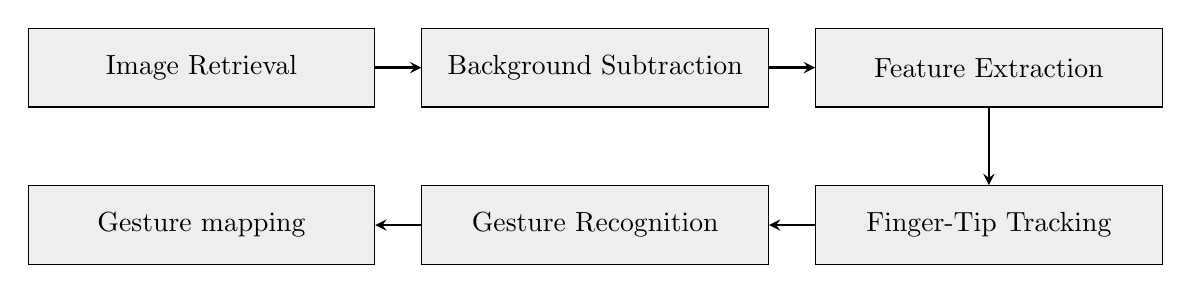
\begin{tikzpicture}[node distance=5cm]
    \node (proc1) [process] {Image Retrieval};
    \node (proc2) [process, right of = proc1] {Background Subtraction};
    \node (proc3) [process, right of = proc2] {Feature Extraction};
    \node (proc4) [process, below of = proc3, yshift = 3cm] {Finger-Tip Tracking};
    \node (proc5) [process, left of = proc4] {Gesture Recognition};
    \node (proc6) [process, left of = proc5] {Gesture mapping};
    \draw [arrow] (proc1) -- (proc2);
    \draw [arrow] (proc2) -- (proc3);
    \draw [arrow] (proc3) -- (proc4);
    \draw [arrow] (proc4) -- (proc5);
    \draw [arrow] (proc5) -- (proc6);
\end{tikzpicture}

\section{Module 1 - Image Retrieval}
The camera feed is retrieved from the user's webcam using the CaptureFromCAM function provided by OpenCV.

\section{Module 2 - Background Subtraction}
The Mixture of Gaussians (MOG) method is used for foreground detection, and once the foreground is detected, we subtract the rest of the image, i. e., the background.

\section{Module 3 - Feature Extraction}
The locations of the fingertips on the screen are detected by finding the Convex hull of the hand and marking the peaks. This process is done in realtime and the extracted location changes with every frame.

\section{Module 4 - Finger-Tip Tracking}
Continuously Adaptive Mean Shift Algorithm (CAMShift) is used to detect the changes from frame to frame. The probability distribution of the first frame is taken as a reference for the second frame, the probability distribution of the second frame is taken for the third frame and so on and so forth.

\section{Module 5 - Gesture Recognition}
The convex hull and convexity defects along with the results of the CAMShift algorithm are used to create a mathematical state of the currently recorded gesture. This state is compared with the states of the saved gestures and the closest candidiate is chosen.

\section{Module 6 - Gesture Mapping}
Once the correct gesture has been identified, the corresponding class object is accessed to procure the GUI function that has been saved for that particular gesture. The function is first executed, and then the daemon starts listening for the next gesture.

\chapter{Data Description}

\section{Data Flow Diagram}

\subsection{Level 0}
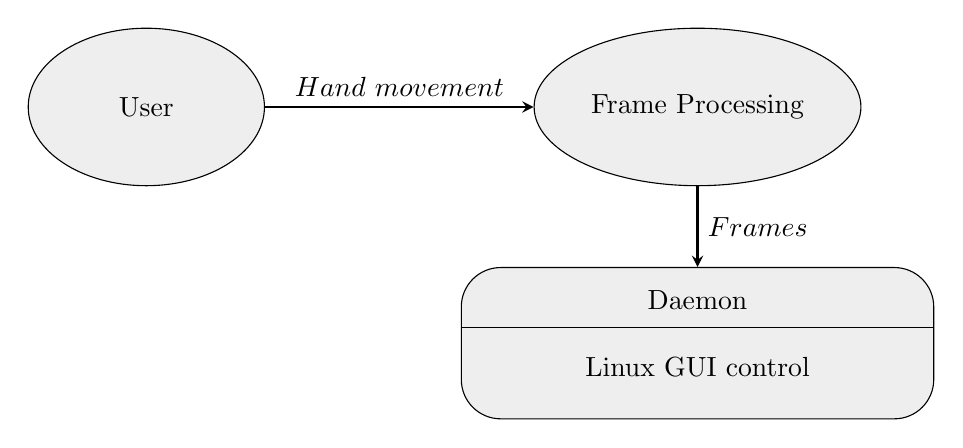
\begin{tikzpicture}[node distance=7cm]
    \node (proc1) [oval]{User};
    \node (proc2) [oval, right of = proc1]{Frame Processing};
    \node (proc3) [process1, below of = proc2, yshift=4cm]{\\Daemon\\\\Linux GUI control\\};
    \draw[arrow] (proc1)--(proc2) node[midway,above,rotate=0] {$Hand\ movement$};
    \draw[arrow] (proc2)--(proc3) node[midway,right,rotate=0] {$Frames$};
    \draw [black] ([yshift=0.2cm]proc3.west)--([yshift=0.2cm]proc3.east);
\end{tikzpicture}
\\
\subsection{Level 1}
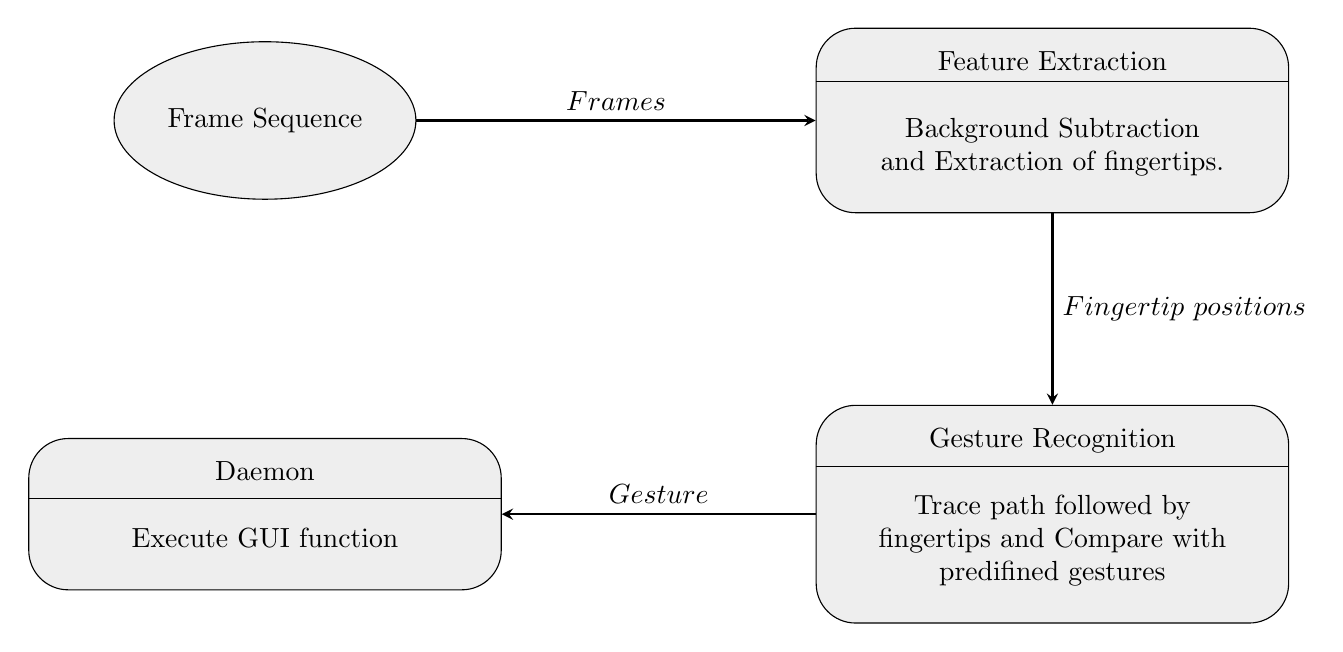
\begin{tikzpicture}[node distance=2cm]
    \node (proc1) [oval]{Frame Sequence};
    \node (proc2) [process1, right of = proc1, xshift=8 cm]{\\Feature Extraction\\\\
    Background Subtraction\\
    and Extraction of fingertips.\\};
    \node (proc3) [process1, below of = proc2, yshift=-3cm]{\\Gesture Recognition\\\\
    Trace path followed by\\
    fingertips and Compare with\\
    predifined gestures\\};
    \node (proc4) [process1, left of = proc3, xshift=-8cm]{\\Daemon\\\\Execute GUI function\\};
    \draw[arrow] (proc1)--(proc2) node[midway,above,rotate=0] {$Frames$};
    \draw[arrow] (proc2)--(proc3) node[midway,right,rotate=0]{$Fingertip\ positions$};
    \draw[arrow] (proc3)--(proc4) node[midway,above,rotate=0] {$Gesture$};
    \draw [black] ([yshift=0.5cm]proc2.west)--([yshift=0.5cm]proc2.east);
    \draw [black] ([yshift=0.6cm]proc3.west)--([yshift=0.6cm]proc3.east);
    \draw [black] ([yshift=0.2cm]proc4.west)--([yshift=0.2cm]proc4.east);
\end{tikzpicture}

\subsection{Level 2}
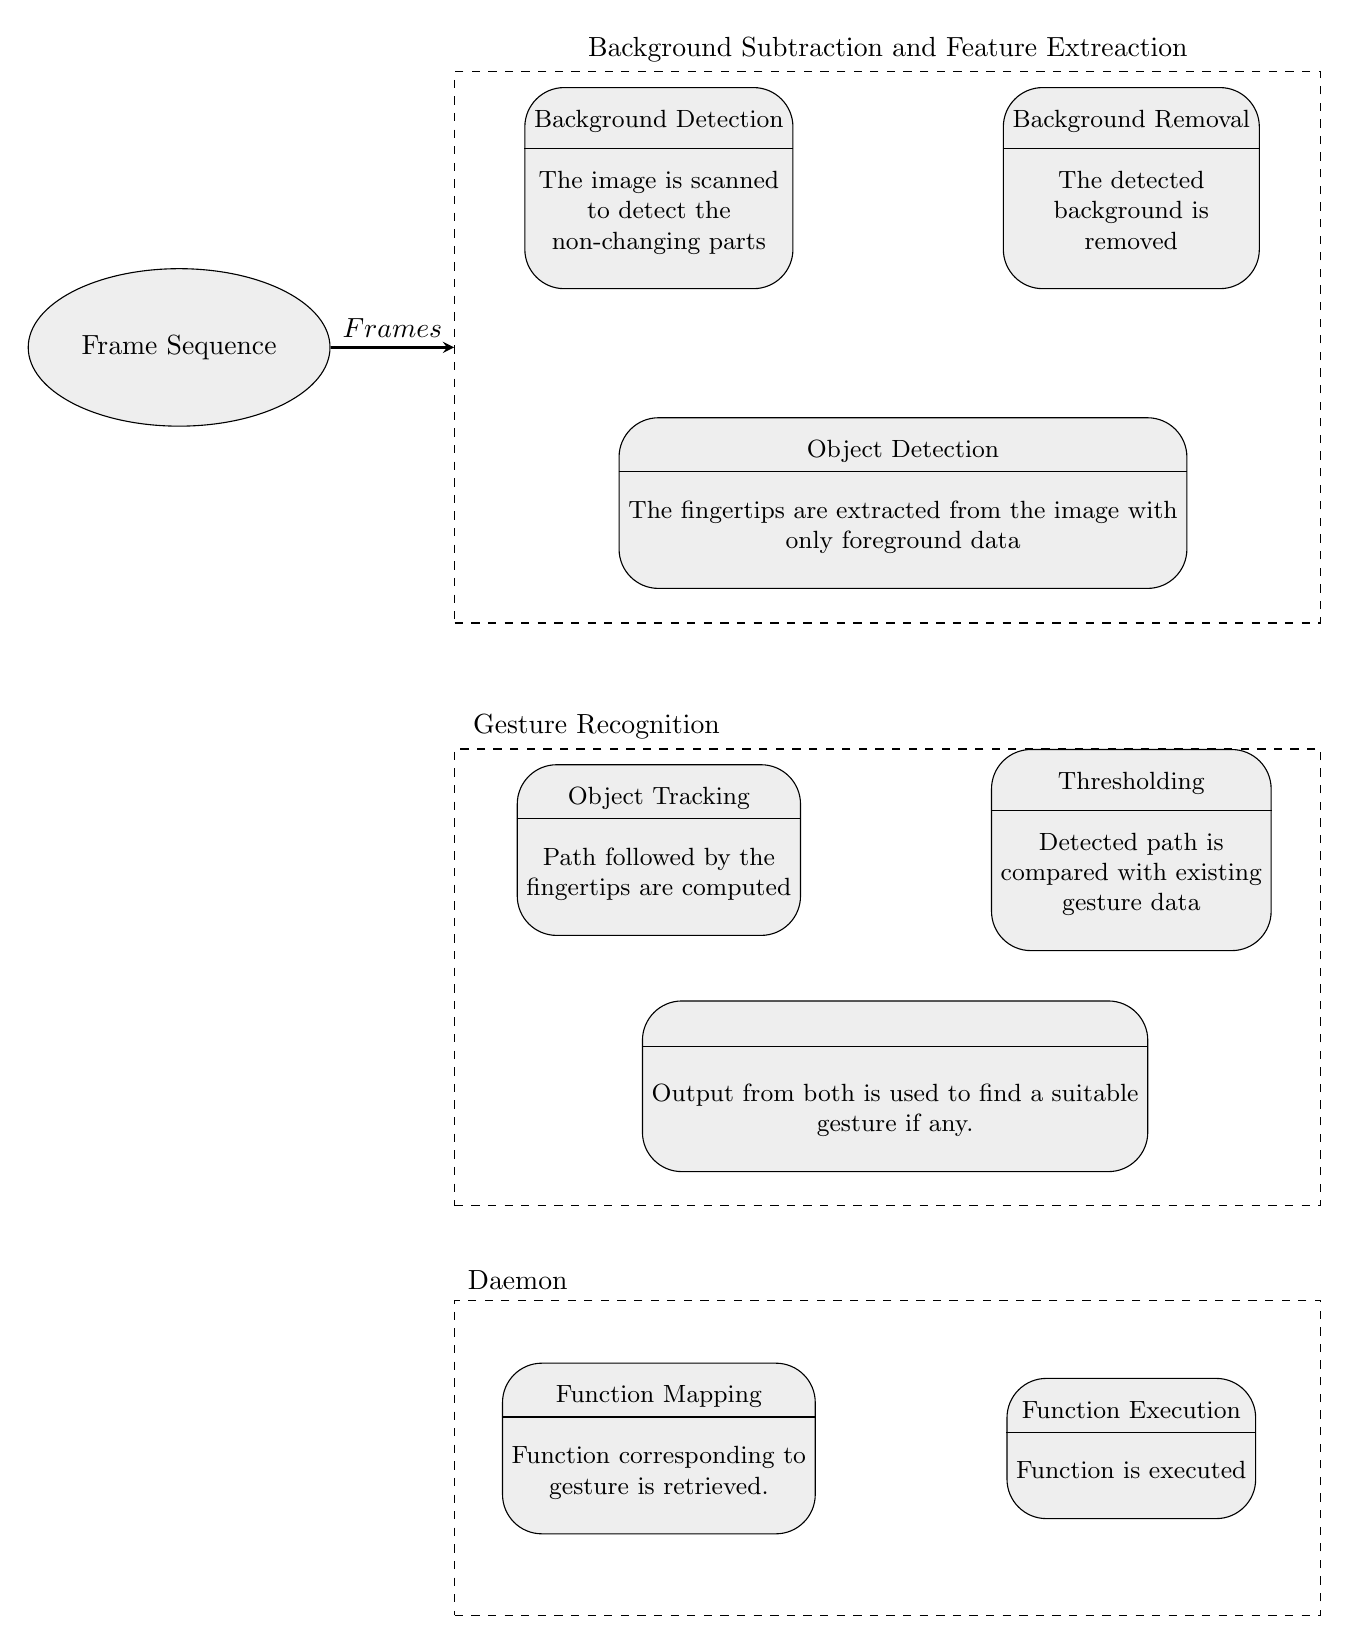
\begin{tikzpicture}[node distance=0cm]
    \node (proc1) [oval]{Frame Sequence};

    \node (over1) [overlay, label=above:Background Subtraction and Feature Extreaction, minimum width = 11cm, minimum height = 7cm, right of = proc1, xshift=9cm]{};

    \node (proc2) [process2, below=of over1.north west, xshift=2.6cm, yshift=-0.2cm]{\\Background Detection\\\\
    The image is scanned\\
    to detect the\\
    non-changing parts\\};


    \node (proc3) [process2, right of = proc2, xshift=6cm]{\\Background Removal\\\\
    The detected\\
    background is\\
    removed\\};

    \node (proc4) [process2, left of = proc3, xshift=-2.9cm, yshift=-4cm]{\\Object Detection\\\\
    The fingertips are extracted from the image with\\
    only foreground data\\};

    \draw[arrow] (proc1)--(over1) node[midway,above,rotate=0] {$Frames$};
    \draw [black] ([yshift=0.5cm]proc2.west)--([yshift=0.5cm]proc2.east);
    \draw [black] ([yshift=0.5cm]proc3.west)--([yshift=0.5cm]proc3.east);
    \draw [black] ([yshift=0.4cm]proc4.west)--([yshift=0.4cm]proc4.east);

    \node (over2) [overlay, label={[xshift=-3.7cm]Gesture Recognition}, minimum width = 11cm, minimum height = 5.8cm, right of = over1, yshift=-8cm]{};

    \node (proc5) [process2, below=of over2.north west, xshift=2.6cm, yshift=-0.2cm]{\\Object Tracking\\\\
    Path followed by the\\
    fingertips are computed\\};

    \node (proc6) [process2, right of = proc5, xshift=6cm]{\\Thresholding\\\\
    Detected path is\\
    compared with existing\\
    gesture data\\};

    \node (proc7) [process2, left of = proc6, xshift=-3cm, yshift=-3cm]{\\\\\\
    Output from both is used to find a suitable\\
    gesture if any.\\};

    \draw [black] ([yshift=0.4cm]proc5.west)--([yshift=0.4cm]proc5.east);
    \draw [black] ([yshift=0.5cm]proc6.west)--([yshift=0.5cm]proc6.east);
    \draw [black] ([yshift=0.5cm]proc7.west)--([yshift=0.5cm]proc7.east);

    \node (over3) [overlay, label={[xshift=-4.7cm]Daemon}, minimum width = 11cm, minimum height = 4cm, right of = over2, yshift=-6.1cm]{};

    \node (proc8) [process2, below=of over3.north west, xshift=2.6cm, yshift=-0.8cm]{\\Function Mapping\\\\
    Function corresponding to\\
    gesture is retrieved.\\};

    \node (proc9) [process2, right of = proc8, xshift=6cm]{\\Function Execution\\\\
    Function is executed\\};

    \draw [black] ([yshift=0.4cm]proc8.west)--([yshift=0.4cm]proc8.east);
    \draw [black] ([yshift=0.2cm]proc9.west)--([yshift=0.2cm]proc9.east);

\end{tikzpicture}

\section{Use case diagram}
\begin{center}
    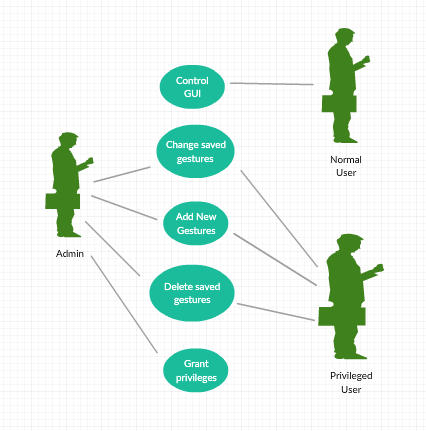
\includegraphics{usecase.png}
\end{center}
\section{Class diagram}
\begin{center}
    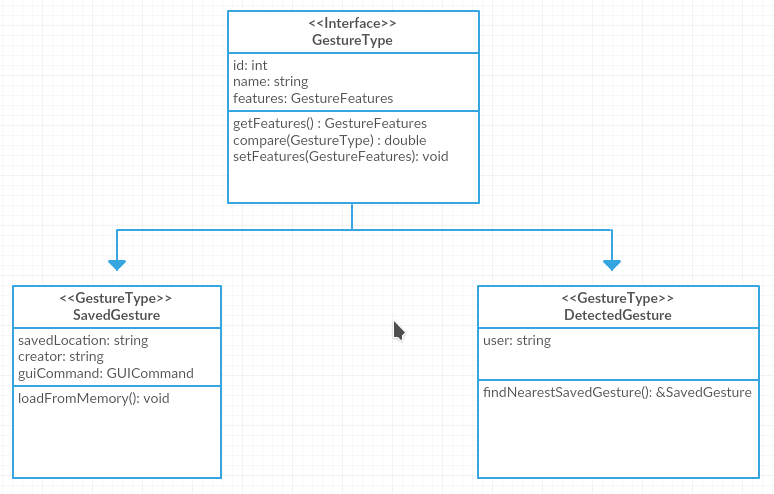
\includegraphics[scale=0.8]{classdiagram.png}
    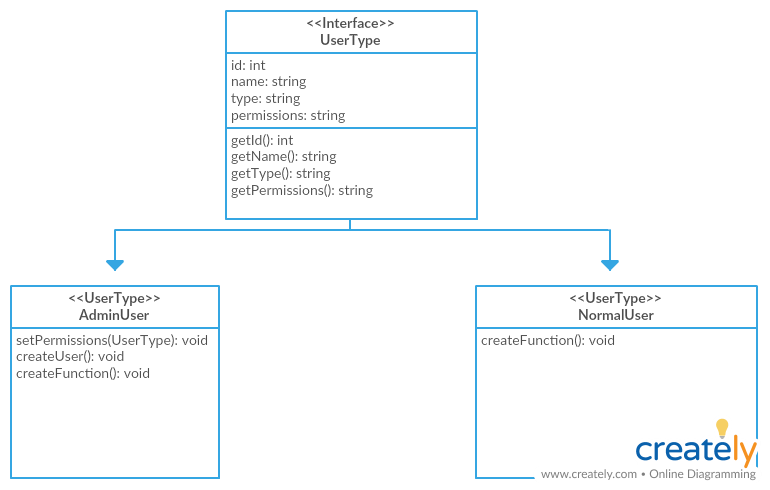
\includegraphics[scale=0.8]{UserClass.png}
\end{center}
\section{Activity diagram}
\begin{center}
    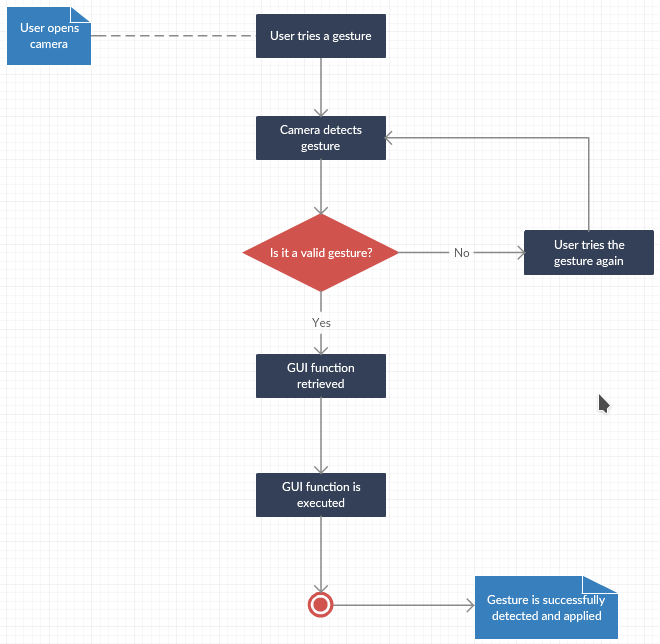
\includegraphics[scale=0.8]{activitydiagram.png}
\end{center}

\chapter{Algorithms}
Explain the pseudocodes of the algorithms that will be used in the implementation of the project.
\section{Overall algorithm}
\begin{itemize}
    \item Input: A set of contiguous video frames
    \item Processing:
    \begin{enumerate}
        \item Calculate the foreground using MOG2 background subtraction algorithm.
        \item Detect the fingertips using the Convex Hull algorithm.
        \item Track the finger gesture using Continuously Adaptive Mean Shift (CAMshift) algorithm.
        \item Save the above tracked graph to a DetectedGesture object.
        \item Find the closest SavedGesture object and execute the GUI function.
    \end{enumerate}
    \item Output: The mapped GUI function
\end{itemize}
\section{Background subtraction}
\begin{enumerate}
    \item Transform video into frames
    \item Estimate the background by using Frame Different Method
    \item Calculate foreground area by applying: Foreground = Frame - Estimated background
    \item Apply the threshold to find the output
\end{enumerate}
\section{Convex Hull}
\begin{itemize}
    \item Input: a list P of points in the plane.
    \item Precondition: There must be at least 3 points.
    \item Processing:
    \begin{enumerate}
        \item Initialize p as leftmost point.
        \item Do following while we don’t come back to the first (or leftmost) point.
        \begin{enumerate}
            \item The next point q is the point such that the triplet (p, q, r) is counterclockwise for any other point r.
            \item next[p] = q (Store q as next of p in the output convex hull).
            \item p = q (Set p as q for next iteration).
        \end{enumerate}
    \end{enumerate}
    \item Output: List of Convex Hull peaks
\end{itemize}
\section{CAMShift}
\begin{itemize}
    \item Input: Sequence of video frames
    \item Processing:
    \begin{enumerate}
        \item Set the calculation region of the probability distribution equal to the whole frame.
        \item Choose the initial location of the two-dimensional mean shift search window.
        \item Calculate the colour probability distribution in the 2D region centred on the search window location in an area slightly larger than the mean shift window size.
        \item Perform the search of the maximum density probability using the mean shift parameter for convergence or for setting the number of iterations. Store the zero moment (area or size) and middle position.
        \item For the next video frame, place the search window in the middle position fixed in step 4, and set the window size in conformity to the last moment. Go to step 3. 
    \end{enumerate}
\end{itemize}
\begin{thebibliography}{999}
\addcontentsline{toc}{chapter}{References}

\bibitem{} 
\bibitem{}

\bibitem{} 

\bibitem{} 

\bibitem{} 

\bibitem{} 



\end{thebibliography}

\end{document}
